\begin{comment}
\documentclass[10pt]{article}
\usepackage{fullpage, graphicx, url}
\setlength{\parskip}{1ex}
\setlength{\parindent}{0ex}
\title{wguide1}
\begin{document}


\begin{tabular}{ccc}
The Alternative Csound Reference Manual & & \\
Previous & &Next

\end{tabular}

%\hline 
\end{comment}
\section{wguide1}
wguide1�--� A simple waveguide model consisting of one delay-line and one first-order lowpass filter. \subsection*{Description}


  A simple waveguide model consisting of one delay-line and one first-order lowpass filter. 
\subsection*{Syntax}


 ar \textbf{wguide1}
 asig, xfreq, kcutoff, kfeedback
\subsection*{Performance}


 \emph{asig}
 -- the input of excitation noise. 


 \emph{xfreq}
 -- the frequency (i.e. the inverse of delay time) Changed to x-rate in Csound version 3.59. 


 \emph{kcutoff}
 -- the filter cutoff frequency in Hz. 


 \emph{kfeedback}
 -- the feedback factor. 


 \emph{wguide1}
 is the most elemental waveguide model, consisting of one delay-line and one first-order lowpass filter. 


  Implementing waveguide algorithms as opcodes, instead of orc instruments, allows the user to set \emph{kr}
 different than \emph{sr}
, allowing better performance particulary when using real-time. 


 


 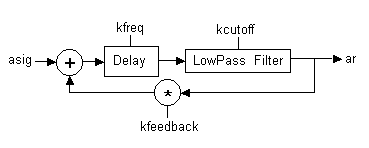
\includegraphics[scale=1]{wguide1} 


 wguide1.
\subsection*{Examples}


  Here is an example of the wguide1 opcode. It uses the files \emph{wguide1.orc}
 and \emph{wguide1.sco}
. 


 \textbf{Example 1. Example of the wguide1 opcode.}

\begin{lstlisting}
/* wguide1.orc */
; Initialize the global variables.
sr = 44100
kr = 4410
ksmps = 10
nchnls = 1

; Instrument #1 - a simple noise waveform.
instr 1
  ; Generate some noise.
  asig noise 20000, 0.5

  out asig
endin

; Instrument #2 - a waveguide example.
instr 2
  ; Generate some noise.
  asig noise 20000, 0.5

  ; Run it through a wave-guide model.
  kfreq init 200
  kcutoff init 3000
  kfeedback init 0.8
  awg1 wguide1 asig, kfreq, kcutoff, kfeedback

  out awg1
endin
/* wguide1.orc */
        
\end{lstlisting}
\begin{lstlisting}
/* wguide1.sco */
; Play Instrument #1 for 2 seconds.
i 1 0 2
; Play Instrument #2 for 2 seconds.
i 2 2 2
e
/* wguide1.sco */
        
\end{lstlisting}
\subsection*{See Also}


 \emph{wguide2}

\subsection*{Credits}


 


 


\begin{tabular}{ccc}
Author: Gabriel Maldonado &Italy &October 1998

\end{tabular}



 


 Example written by Kevin Conder.


 New in Csound version 3.49
%\hline 


\begin{comment}
\begin{tabular}{lcr}
Previous &Home &Next \\
wgpluck2 &Up &wguide2

\end{tabular}


\end{document}
\end{comment}
